\section{Auswertung}
\label{sec:Auswertung}

\subsection{Literaturwerte}

Die Ordnungszahlen der Stoffe, die im Versuch untersucht werden sind in
Tabelle \ref{tab:litwerte} aufgezählt.
Die Werte für die Lichtgeschwindigkeit $c$, die Elementarladung $e$, die
Feinstrukturkonstante $\alpha$ und das Plancksche Wirkungsquantum $h$ werden aus
\cite{Codata} entnommen.

\subsection{Überprüfung der Bragg Bedingung}

In Tabelle \ref{tab:braggbed} sind die Messwerte zur Überprüfung der braggschen
Bedingung dargestellt. Diese sind in Abbildung \ref{fig:braggbed} als Graph
aufgetragen.
Das Maximum der Kurve liegt bei
\begin{align}
  \theta_\text{mess} = \SI{28.4}{\degree}.
\end{align}
Der Sollwert für das Maximum lautet
\begin{equation}
  \theta_\text{soll} = \SI{28}{\degree}.
\end{equation}

\subsection{Das Emissionsspektrum einer CU-Röntgenröhre}

In Tabelle \ref{tab:emission1}, \ref{tab:emission2}, \ref{tab:emission3} und
\ref{tab:emission4} sind die Messwerte zur Bestimmung des
Emissionsspektrum der CU-Röntgenröhre abgebildet. Der zugehörige Graph ist
ist in Abbildung \ref{fig:emission} dargestellt.
Der Grenzwinkel befindet sich bei
\begin{equation}
  \theta_\text{CU} = \SI{8.8}{\degree}.
\end{equation}
Mit der Bragg'schen Bedingung folgt dann die minimale Wellenlänge
\begin{equation}
  \lambda_\text{CU} = \SI{0.0616}{\nano\meter}
\end{equation}
bzw. die maximale Energie, bei der die Elektronen vollständig abgebremst werden,
\begin{equation}
  E_\text{CU} = \SI{20.1197}{\kilo\electronvolt}.
\end{equation}
In den Abbildungen \ref{fig:emissionkalpha} und \ref{fig:emissionkbeta} sind
jeweils die Messwerte an der $K_\alpha$- und $K_\beta$- Linie des
Emissionsspektrums abgebildet. Diese werden jeweils durch ein Polynom zweiten
Grades angenähert.
Die Hochpunkte der Parabeln sind bei
\begin{align}
  \theta_\alpha = & \SI{44.2196}{\degree} \\
  \theta_\beta = & \SI{39.6213}{\degree}.
\end{align}
Daraus folgen die Halbwerte
\begin{align}
  \theta_{\alpha 1} = & \SI{43.7517}{\degree} \\
  \theta_{\alpha 2} = & \SI{44.6875}{\degree} \\
  \theta_{\beta 1} = & \SI{39.0093}{\degree} \\
  \theta_{\beta 2} = & \SI{40.2333}{\degree}.
\end{align}
Durch bilden der Differenzen ergeben sich die Halbwertsbreiten der
$K_\alpha$- und $K_\beta$- Linie
\begin{align}
  \increment \theta_\alpha = & \SI{0.9358}{\degree} \\
  \increment \theta_\beta = & \SI{1.2240}{\degree}.
\end{align}
Die Energieauflösung ergibt sich aus dem Mittelwert der Energieauflösungen
der $K_\alpha$- und $K_\beta$- Linie
\begin{equation}
  \increment E = \frac{1}{2}(\increment E_\alpha + \increment E_\beta) \pm
  \sqrt{(\increment E_\alpha - \bar{E})^2 + (\increment E_\beta - \bar{E})^2}
  = \SI{172(138)}{\electronvolt}.
\end{equation}
Die Differenz der Energien an der $K_\alpha$- und $K_\beta$-Linien ist
\begin{align}
  E_\text{CU,mess} = \SI{0.9041}{\kilo\electronvolt}.
\end{align}
Daraus folgt mit
\begin{align}
  \sigma_K = Z - \sqrt{\frac{E}{R_\infty}- \frac{\alpha^2}{4}z^4}
  \label{eqn:sigmaK}
\end{align}
die Abschirmkonstante an der K-Kante von Kupfer
\begin{align}
  \sigma_\text{K,CU,mess} = 21.4460
\end{align}

\subsection{Absorptionsspektren verschiedener Stoffe}

\subsubsection{Germanium}

Die Messwerte der Germaniumprobe sind in Tabelle \ref{tab:germanium1} und
\ref{tab:germanium2} abgebildet
und als Graph in Abbildung \ref{fig:germanium} aufgetragen.
Die gemessene K-Kante befindet sich bei
\begin{equation}
  2\theta_\text{Ge} = \SI{32.4}{\degree}.
\end{equation}
Mit der Bragg'schen Bedingung \eqref{eqn:braggbed} folgt dann für die
Wellenlänge
\begin{equation}
  \lambda_\text{Ge} = \SI{0.1124}{\nano\meter}.
\end{equation}
Mit der Formel
\begin{equation}
  E = \frac{c h}{\lambda}
  \label{eqn:energielambda}
\end{equation}
folgt der Energiewert an der K-Kante für Germanium
\begin{equation}
  E_\text{Ge,mess} = \SI{11.0328}{\kilo\electronvolt}.
\end{equation}
Mit \eqref{eqn:sigmaK} folgt die Abschirmzahl an der K-Kante von Germanium
\begin{align}
  \sigma_\text{K,Ge,mess} = 3.7639.
\end{align}

\subsubsection{Brom}

Die Messwerte der Bromprobe sind in Tabelle \ref{tab:brom1} und \ref{tab:brom2}
dargestellt und als
Graph in der Abbildung \ref{fig:brom} aufgetragen.
Die gemessene K-Kante befindet sich bei
\begin{equation}
  2\theta_\text{Br} = 25.4 .
\end{equation}
Für die Wellenlänge folgt mit \eqref{eqn:braggbed}
\begin{equation}
  \lambda_\text{Br} = \SI{0.0886}{\nano\meter}.
\end{equation}
Daraus ergibt sich mit Hilfe der Formel \eqref{eqn:energielambda}
der Wert am Energieübergang
\begin{equation}
  E_\text{Br,mess} = \SI{14.0008}{\kilo\electronvolt}.
\end{equation}
Mit \eqref{eqn:sigmaK} folgt die Abschirmkonstante an der K-Kante von Brom
\begin{align}
  \sigma_\text{K,Br,mess} = 3.2274.
\end{align}

\subsubsection{Zirkonium}

Die Messwerte für Zirkonium sind in den Tabellen \ref{tab:zirkonium1} und
\ref{tab:zirkonium2} dargestellt und
in Abbildung \ref{fig:zirkonium} als Graph aufgetragen.
Die K-Kante wird bei
\begin{equation}
  2\theta_\text{Zr} = \SI{18.8}{\degree}
\end{equation}
gemessen.
Daraus folgt mit \eqref{eqn:braggbed} die Wellenlänge
\begin{equation}
  \lambda_\text{Zr} = \SI{0.0658}{\nano\meter}.
\end{equation}
Mit \eqref{eqn:energielambda} folgt der Energiewert von Zirkonium an der
K-Kante
\begin{align}
  E_\text{Zr,mess} = \SI{18.8459}{\kilo\electronvolt}.
\end{align}
Die Abschirmkostante ergibt sich mit der Formel \eqref{eqn:sigmaK}
\begin{align}
  \sigma_\text{K,Zr,mess} = 3.2352.
\end{align}

\subsubsection{Bismuth}

In Tabelle \ref{tab:bismuth1} und \ref{tab:bismuth2} sind die Messwerte der
Bismuthprobe abgebildet.
Diese sind in Abbildung \ref{fig:bismuth} als Graph aufgetragen.
Die Messung ergibt einen Winkel von
\begin{align}
  2\theta_\text{Bi,LII} = \SI{21.4}{\degree}
\end{align}
an der LII-Kante und einen Winkel von
\begin{align}
  2\theta_\text{Bi,LIII} = \SI{25.6}{\degree}
\end{align}
an der LIII-Kante.
Daraus ergeben sich mit \eqref{eqn:braggbed} die Wellenlängen
\begin{align}
  \lambda_\text{Bi,LII} = \SI{0.0748}{\nano\meter}
\end{align}
und
\begin{align}
  \lambda_\text{Bi,LIII} = \SI{0.0892}{\nano\meter}.
\end{align}
Mit \eqref{eqn:energielambda} folgt der Energiedifferenzwert der L-Kanten von
Bismuth
\begin{align}
  E_\text{Bi,mess} = \SI{2.7850}{\kilo\electronvolt}.
\end{align}
Daraus ergibt sich mit \eqref{eqn:sigmal} die Abschirmkonstante der L-Schale
von Bismuth
\begin{align}
  \sigma_\text{L,Bi,mess} = 0.9265.
\end{align}

\subsection{Das Moseleysche Gesetz}

In Abbildung \ref{fig:moseley} sind die berechneten Absorptionsenergien und die
Kernladungszahlen für Germanium, Brom und Zirkonium in einem
$\sqrt{E_k}-Z$-Diagramm dargestellt. Durch die Werte wird eine Ausgleichsgerade
gelegt, die ausgegebene Steigung beträgt
\begin{align}
  m = \num{0.25(1)}.
\end{align}
Daraus ergibt sich die Rydbergkonstante
\begin{align}
  R_\text{\infty, mess} = \SI{22(2)}{\per\meter}.
\end{align}

\begin{figure}
  \centering
  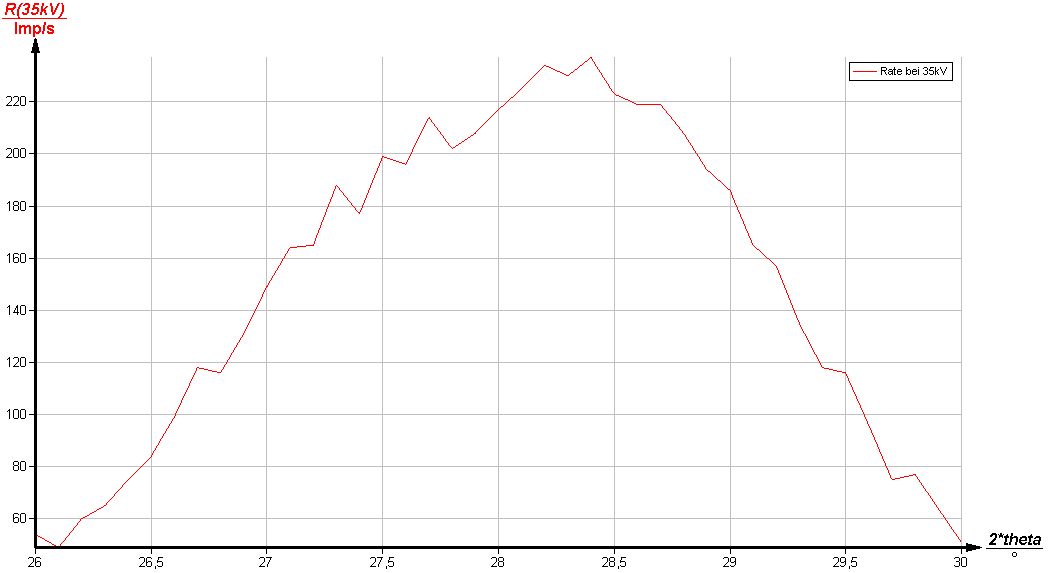
\includegraphics[height=9cm]{Daten/braggbedingung.png}
  \caption{Graph zur Überprüfung der Bragg Bedingung. Es sind die Impulse pro
  Sekunde gegen den Winkel aufgetragen.}
  \label{fig:braggbed}
\end{figure}

\begin{figure}
  \centering
  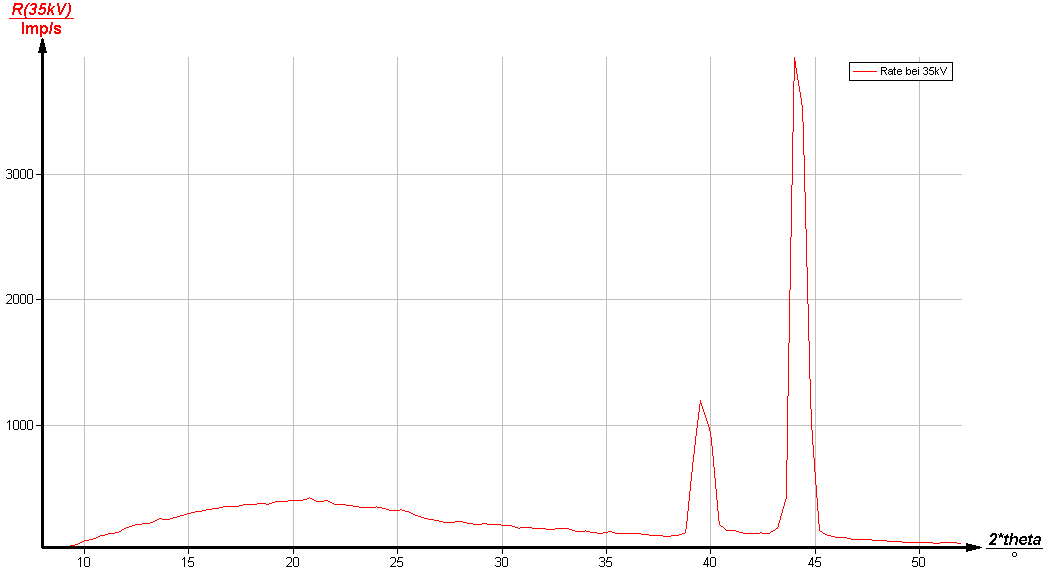
\includegraphics[height=8cm]{Daten/emissionsspektrum.png}
  \caption{Graph des Emissionsspektrums der CU-Röntgenröhre. Es sind die
  Impulse pro Sekunde gegen den Winkel aufgetragen.}
  \label{fig:emission}
\end{figure}

\begin{figure}
  \centering
  \includegraphics[height=8cm]{build/emissionsspektrumKbetha.pdf}
  \caption{Messwerte der $K_\alpha$-Linie des Emissionsspektrums der
  CU-Röntgenröhre und Ausgleichspolynom. Es sind die
  Impulse pro Sekunde gegen den Winkel aufgetragen.}
  \label{fig:emissionkalpha}
\end{figure}

\begin{figure}
  \centering
  \includegraphics[height=8cm]{build/emissionsspektrumKalpha.pdf}
  \caption{Messwerte der $K_\beta$-Linie des Emissionsspektrums der
  CU-Röntgenröhre und Ausgleichspolynom. Es sind die Impulse pro Sekunde
  gegen den Winkel aufgetragen.}
  \label{fig:emissionkbeta}
\end{figure}

\begin{figure}
  \centering
  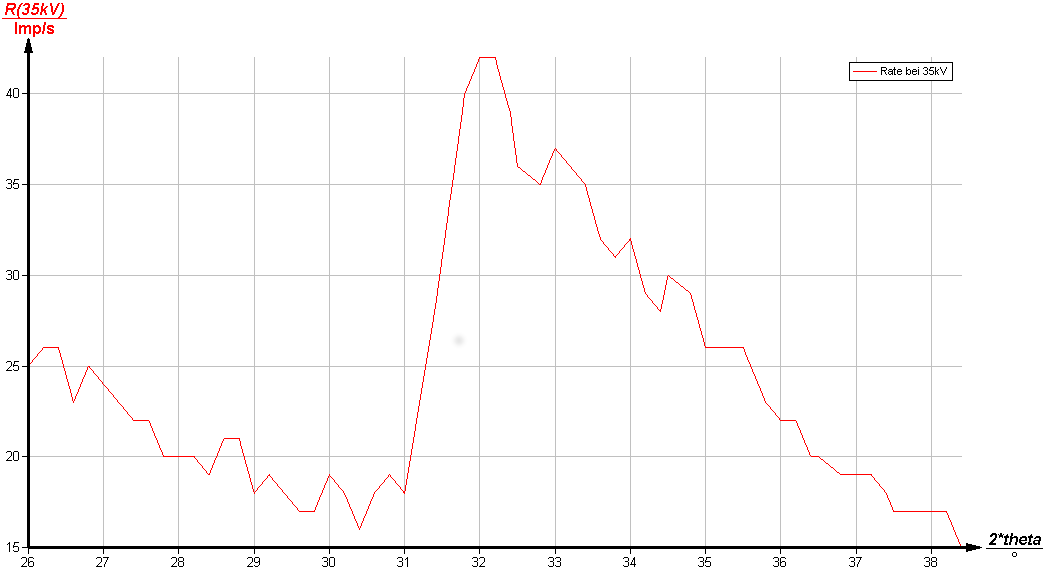
\includegraphics[height=8cm]{Daten/germanium.png}
  \caption{Graph der Messwerte des Absorptionsspektrums der Germaniumprobe. Es
  sind die Impulse pro Sekunde gegen den Winkel aufgetragen.}
  \label{fig:germanium}
\end{figure}

\begin{figure}
  \centering
  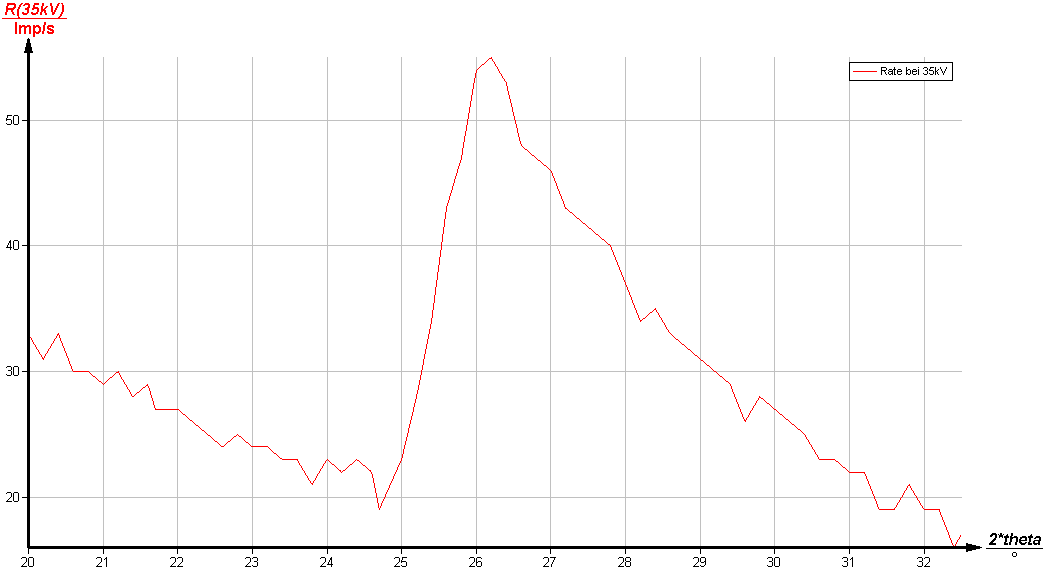
\includegraphics[height=8cm]{Daten/brom.png}
  \caption{Graph der Messwerte des Absorptionsspektrums der Bromprobe. Es
  sind die Impulse pro Sekunde gegen den Winkel aufgetragen.}
  \label{fig:brom}
\end{figure}

\begin{figure}
  \centering
  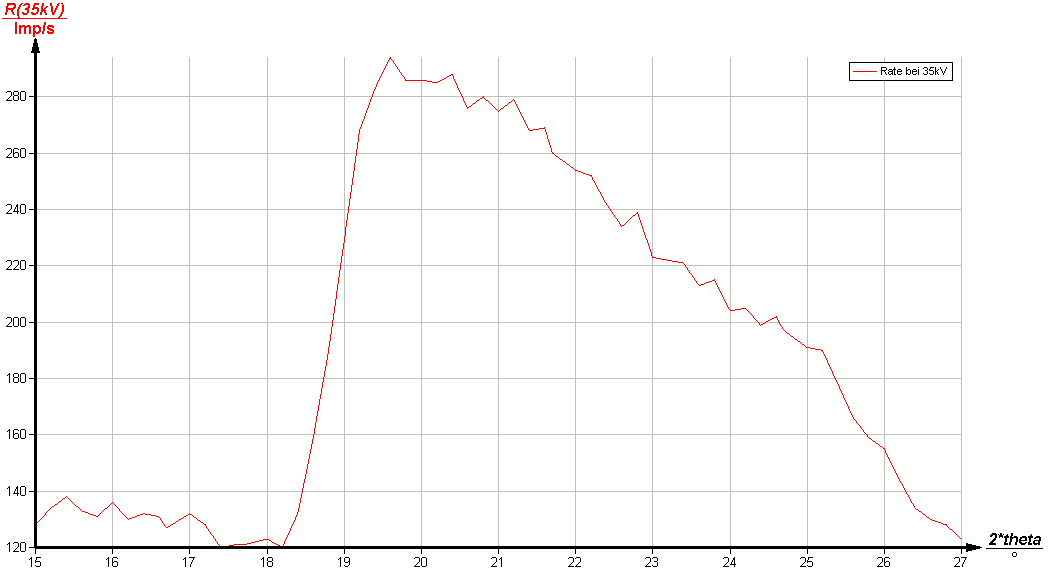
\includegraphics[height=8cm]{Daten/zirkonium.png}
  \caption{Graph der Messwerte des Absorptionsspektrums der Zirkoniumprobe. Es
  sind die Impulse pro Sekunde gegen den Winkel aufgetragen.}
  \label{fig:zirkonium}
\end{figure}

\begin{figure}
  \centering
  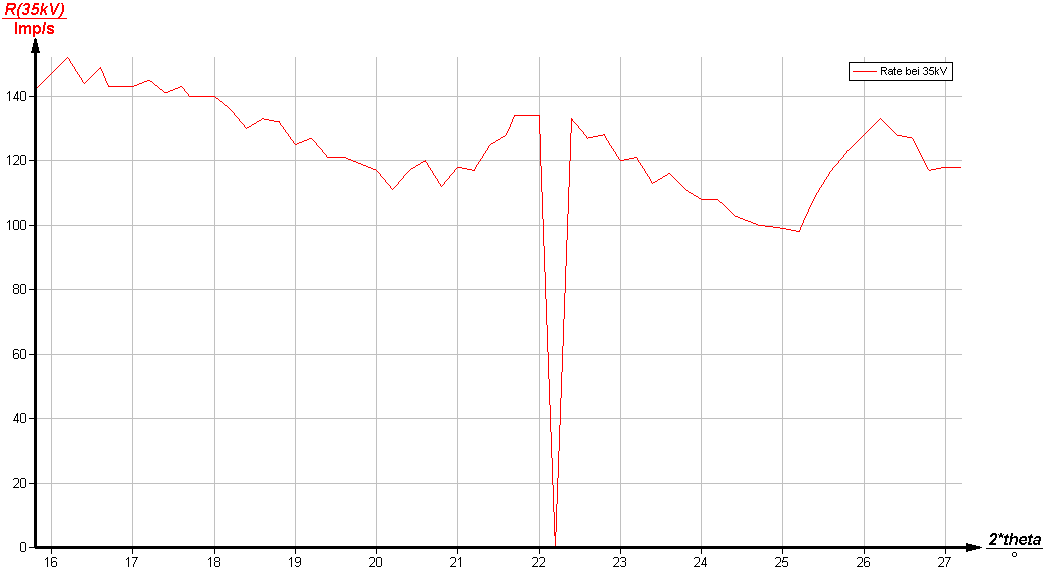
\includegraphics[height=8cm]{Daten/bismuth.png}
  \caption{Graph der Messwerte des Absorptionsspektrums der Bismuthprobe. Es
  sind die Impulse pro Sekunde gegen den Winkel aufgetragen.}
  \label{fig:bismuth}
\end{figure}

\begin{figure}
  \centering
  \includegraphics[height=8cm]{build/Moseley.pdf}
  \caption{Graph zur Bestimmung der Rydbergkonstante. Es ist $\sqrt{E_k}$ gegen
  Z aufgetragen.}
  \label{fig:moseley}
\end{figure}

\begin{table}[h]
  \centering
  \begin{tabular}{S S}
    \toprule
    {$\theta/\si{\degree}$} & {$Imp/\si{\second}$}\\
    \midrule
    26.0 & 54.0\\
    26.1 & 49.0\\
    26.2 & 60.0\\
    26.3 & 65.0\\
    26.4 & 75.0\\
    26.5 & 84.0\\
    26.6 & 99.0\\
    26.7 & 118.0\\
    26.8 & 116.0\\
    26.9 & 131.0\\
    27.0 & 149.0\\
    27.1 & 164.0\\
    27.2 & 165.0\\
    27.3 & 188.0\\
    27.4 & 177.0\\
    27.5 & 199.0\\
    27.6 & 196.0\\
    27.7 & 214.0\\
    27.8 & 202.0\\
    27.9 & 208.0\\
    28.0 & 217.0\\
    28.1 & 225.0\\
    28.2 & 234.0\\
    28.3 & 230.0\\
    28.4 & 237.0\\
    28.5 & 223.0\\
    28.6 & 219.0\\
    28.7 & 219.0\\
    28.8 & 208.0\\
    28.9 & 194.0\\
    29.0 & 186.0\\
    29.1 & 165.0\\
    29.2 & 157.0\\
    29.3 & 135.0\\
    29.4 & 118.0\\
    29.5 & 116.0\\
    29.6 & 96.0\\
    29.7 & 75.0\\
    29.8 & 77.0\\
    29.9 & 64.0\\
    30.0 & 51.0\\
    \bottomrule
  \end{tabular}
  \caption{Messwerte zur Überprüfung der Bragg Bedingung. Es sind die
  Impulse pro Sekunde gegen den Winkel aufgetragen.}
  \label{tab:braggbed}
\end{table}

\begin{table}[h]
  \centering
  \begin{tabular}{S S}
    \toprule
    {$\theta/\si{\degree}$} & {$Imp\si{\second}$}\\
    \midrule
    8.0	& 26.0\\
    8.4	& 26.0\\
    8.8	& 26.0\\
    9.2	& 35.0\\
    9.6	& 46.0\\
    10.0 & 78.0\\
    10.4 & 92.0\\
    10.8 & 118.0\\
    11.2 & 136.0\\
    11.6 & 145.0\\
    12.0 & 182.0\\
    12.4 & 205.0\\
    12.8 & 214.0\\
    13.2 & 223.0\\
    13.6 & 256.0\\
    14.0 & 247.0\\
    14.4 & 269.0\\
    14.8 & 286.0\\
    15.2 & 306.0\\
    15.6 & 316.0\\
    16.0 & 331.0\\
    16.4 & 337.0\\
    16.7 & 353.0\\
    17.2 & 349.0\\
    17.6 & 365.0\\
    18.0 & 367.0\\
    18.4 & 376.0\\
    18.8 & 372.0\\
    \bottomrule
  \end{tabular}
  \caption{Messwerte zur Bestimmung des Emissionsspektrums (1). Es sind die
  Impulse pro Sekunde gegen den Winkel aufgetragen.}
  \label{tab:emission1}
\end{table}

\begin{table}[h]
  \centering
  \begin{tabular}{S S}
    \toprule
    {$\theta/\si{\degree}$} & {$Imp\si{\second}$}\\
    \midrule
    19.2 & 391.0\\
    19.6 & 394.0\\
    20.0 & 402.0\\
    20.4 & 400.0\\
    20.8 & 421.0\\
    21.2 & 389.0\\
    21.6 & 400.0\\
    22.0 & 371.0\\
    22.4 & 369.0\\
    22.8 & 358.0\\
    23.2 & 348.0\\
    23.6 & 342.0\\
    24.0 & 349.0\\
    24.4 & 336.0\\
    24.7 & 320.0\\
    25.2 & 326.0\\
    25.6 & 305.0\\
    26.0 & 274.0\\
    26.4 & 255.0\\
    26.8 & 244.0\\
    27.2 & 229.0\\
    27.6 & 225.0\\
    28.0 & 235.0\\
    28.4 & 218.0\\
    28.8 & 210.0\\
    29.2 & 215.0\\
    29.6 & 208.0\\
    30.0 & 205.0\\
    \bottomrule
  \end{tabular}
  \caption{Messwerte zur Bestimmung des Emissionsspektrums (2). Es sind die
  Impulse pro Sekunde gegen den Winkel aufgetragen.}
  \label{tab:emission2}
\end{table}


\begin{table}[h]
  \centering
  \begin{tabular}{S S}
    \toprule
    {$\theta/\si{\degree}$} & {$Imp\si{\second}$}\\
    \midrule
    30.4 & 202.0\\
    30.8 & 180.0\\
    31.2 & 189.0\\
    31.6 & 176.0\\
    32.0 & 174.0\\
    32.4 & 172.0\\
    32.8 & 176.0\\
    33.2 & 174.0\\
    33.6 & 152.0\\
    34.0 & 158.0\\
    34.4 & 142.0\\
    34.8 & 141.0\\
    35.2 & 153.0\\
    35.5 & 136.0\\
    36.0 & 140.0\\
    36.4 & 135.0\\
    36.8 & 133.0\\
    37.2 & 121.0\\
    37.5 & 119.0\\
    38.0 & 116.0\\
    38.4 & 122.0\\
    38.8 & 143.0\\
    39.2 & 797.0\\
    39.5 & 1196.0\\
    40.0 & 938.0\\
    40.4 & 212.0\\
    40.8 & 158.0\\
    \bottomrule
  \end{tabular}
  \caption{Messwerte zur Bestimmung des Emissionsspektrums (3). Es sind die
  Impulse pro Sekunde gegen den Winkel aufgetragen.}
  \label{tab:emission3}
\end{table}

\begin{table}[h]
  \centering
  \begin{tabular}{S S}
    \toprule
    {$\theta/\si{\degree}$} & {$Imp\si{\second}$}\\
    \midrule
    41.2 & 158.0\\
    41.5 & 142.0\\
    42.0 & 135.0\\
    42.4 & 142.0\\
    42.8 & 139.0\\
    43.2 & 181.0\\
    43.6 & 414.0\\
    44.0 & 3932.0\\
    44.4 & 3527.0\\
    44.8 & 1040.0\\
    45.2 & 160.0\\
    45.5 & 129.0\\
    46.0 & 108.0\\
    46.4 & 106.0\\
    46.8 & 89.0\\
    47.2 & 87.0\\
    47.6 & 87.0\\
    48.0 & 82.0\\
    48.4 & 78.0\\
    48.8 & 75.0\\
    49.2 & 69.0\\
    49.5 & 63.0\\
    50.0 & 62.0\\
    50.4 & 65.0\\
    50.8 & 60.0\\
    51.2 & 64.0\\
    51.6 & 66.0\\
    52.0 & 56.0\\
    \bottomrule
  \end{tabular}
  \caption{Messwerte zur Bestimmung des Emissionsspektrums (4). Es sind die
  Impulse pro Sekunde gegen den Winkel aufgetragen.}
  \label{tab:emission4}
\end{table}

\begin{table}[h]
  \centering
  \begin{tabular}{S S}
    \toprule
    {$\theta/\si{\degree}$} & {$Imp/\si{\second}$}\\
    \midrule
    26.0 & 25.0 \\
    26.2 & 26.0 \\
    26.4 & 26.0 \\
    26.6 & 23.0 \\
    26.8 & 25.0 \\
    27.0 & 24.0 \\
    27.2 & 23.0 \\
    27.4 & 22.0 \\
    27.6 & 22.0 \\
    27.8 & 20.0 \\
    28.0 & 20.0 \\
    28.2 & 20.0 \\
    28.4 & 19.0 \\
    28.6 & 21.0 \\
    28.8 & 21.0 \\
    29.0 & 18.0 \\
    29.2 & 19.0 \\
    29.4 & 18.0 \\
    29.6 & 17.0 \\
    29.8 & 17.0 \\
    30.0 & 19.0 \\
    30.2 & 18.0 \\
    30.4 & 16.0 \\
    30.6 & 18.0 \\
    30.8 & 19.0 \\
    31.0 & 18.0 \\
    31.2 & 23.0 \\
    \bottomrule
  \end{tabular}
  \caption{Messwerte der Germaniumprobe (1). Es sind die
  Impulse pro Sekunde gegen den Winkel aufgetragen.}
  \label{tab:germanium1}
\end{table}


\begin{table}[h]
  \centering
  \begin{tabular}{S S}
    \toprule
    {$\theta/\si{\degree}$} & {$Imp/\si{\second}$}\\
    \midrule
    31.4 & 28.0 \\
    31.6 & 34.0 \\
    31.8 & 40.0 \\
    32.0 & 42.0 \\
    32.2 & 42.0 \\
    32.4 & 39.0 \\
    32.5 & 36.0 \\
    32.8 & 35.0 \\
    33.0 & 37.0 \\
    33.2 & 36.0 \\
    33.4 & 35.0 \\
    33.6 & 32.0 \\
    33.8 & 31.0 \\
    34.0 & 32.0 \\
    34.2 & 29.0 \\
    34.4 & 28.0 \\
    34.5 & 30.0 \\
    34.8 & 29.0 \\
    35.0 & 26.0 \\
    35.2 & 26.0 \\
    35.4 & 26.0 \\
    35.5 & 26.0 \\
    35.8 & 23.0 \\
    36.0 & 22.0 \\
    36.2 & 22.0 \\
    36.4 & 20.0 \\
    36.5 & 20.0 \\
    36.8 & 19.0 \\
    37.0 & 19.0 \\
    37.2 & 19.0 \\
    37.4 & 18.0 \\
    37.5 & 17.0 \\
    37.8 & 17.0 \\
    38.0 & 17.0 \\
    38.2 & 17.0 \\
    38.4 & 15.0 \\
    \bottomrule
  \end{tabular}
  \caption{Messwerte der Germaniumprobe (2). Es sind die
  Impulse pro Sekunde gegen den Winkel aufgetragen.}
  \label{tab:germanium2}
\end{table}

\begin{table}[h]
  \centering
  \begin{tabular}{S S}
    \toprule
    {$\theta/\si{\degree}$} & {$Imp/\si{\second}$}\\
    \midrule
    20.0 & 33.0 \\
    20.2 & 31.0 \\
    20.4 & 33.0 \\
    20.6 & 30.0 \\
    20.8 & 30.0 \\
    21.0 & 29.0 \\
    21.2 & 30.0 \\
    21.4 & 28.0 \\
    21.6 & 29.0 \\
    21.7 & 27.0 \\
    22.0 & 27.0 \\
    22.2 & 26.0 \\
    22.4 & 25.0 \\
    22.6 & 24.0 \\
    22.8 & 25.0 \\
    23.0 & 24.0 \\
    23.2 & 24.0 \\
    23.4 & 23.0 \\
    23.6 & 23.0 \\
    23.8 & 21.0 \\
    24.0 & 23.0 \\
    24.2 & 22.0 \\
    24.4 & 23.0 \\
    24.6 & 22.0 \\
    24.7 & 19.0 \\
    25.0 & 23.0 \\
    25.2 & 28.0 \\
    25.4 & 34.0 \\
    25.6 & 43.0 \\
    25.8 & 47.0 \\
    26.0 & 54.0 \\
    26.2 & 55.0 \\
    26.4 & 53.0 \\
    \bottomrule
  \end{tabular}
  \caption{Messwerte der Bromprobe (1). Es sind die
  Impulse pro Sekunde gegen den Winkel aufgetragen.}
  \label{tab:brom1}
\end{table}

\begin{table}[h]
  \centering
  \begin{tabular}{S S}
    \toprule
    {$\theta/\si{\degree}$} & {$Imp/\si{\second}$}\\
    \midrule
    26.6 & 48.0 \\
    26.8 & 47.0 \\
    27.0 & 46.0 \\
    27.2 & 43.0 \\
    27.4 & 42.0 \\
    27.6 & 41.0 \\
    27.8 & 40.0 \\
    28.0 & 37.0 \\
    28.2 & 34.0 \\
    28.4 & 35.0 \\
    28.6 & 33.0 \\
    28.8 & 32.0 \\
    29.0 & 31.0 \\
    29.2 & 30.0 \\
    29.4 & 29.0 \\
    29.6 & 26.0 \\
    29.8 & 28.0 \\
    30.0 & 27.0 \\
    30.2 & 26.0 \\
    30.4 & 25.0 \\
    30.6 & 23.0 \\
    30.8 & 23.0 \\
    31.0 & 22.0 \\
    31.2 & 22.0 \\
    31.4 & 19.0 \\
    31.6 & 19.0 \\
    31.8 & 21.0 \\
    32.0 & 19.0 \\
    32.2 & 19.0 \\
    32.4 & 16.0 \\
    32.5 & 17.0 \\
    \bottomrule
  \end{tabular}
  \caption{Messwerte der Bromprobe (2). Es sind die
  Impulse pro Sekunde gegen den Winkel aufgetragen.}
  \label{tab:brom2}
\end{table}

\begin{table}[h]
  \centering
  \begin{tabular}{S S}
    \toprule
    {$\theta/\si{\degree}$} & {$Imp/\si{\second}$}\\
    \midrule
    15.0 & 128.0\\
    15.2 & 134.0\\
    15.4 & 138.0\\
    15.6 & 133.0\\
    15.8 & 131.0\\
    16.0 & 136.0\\
    16.2 & 130.0\\
    16.4 & 132.0\\
    16.6 & 131.0\\
    16.7 & 127.0\\
    17.0 & 132.0\\
    17.2 & 128.0\\
    17.4 & 120.0\\
    17.6 & 121.0\\
    17.7 & 121.0\\
    18.0 & 123.0\\
    18.2 & 120.0\\
    18.4 & 132.0\\
    18.6 & 159.0\\
    18.8 & 190.0\\
    19.0 & 229.0\\
    19.2 & 268.0\\
    19.4 & 283.0\\
    19.6 & 294.0\\
    19.8 & 286.0\\
    20.0 & 286.0\\
    20.2 & 285.0\\
    20.4 & 288.0\\
    20.6 & 276.0\\
    20.8 & 280.0\\
    21.0 & 275.0\\
    \bottomrule
  \end{tabular}
  \caption{Messwerte der Zirkoniumprobe (1). Es sind die
  Impulse pro Sekunde gegen den Winkel aufgetragen.}
  \label{tab:zirkonium1}
\end{table}

\begin{table}[h]
  \centering
  \begin{tabular}{S S}
    \toprule
    {$\theta/\si{\degree}$} & {$Imp/\si{\second}$}\\
    \midrule
    21.2 & 279.0\\
    21.4 & 268.0\\
    21.6 & 269.0\\
    21.7 & 260.0\\
    22.0 & 254.0\\
    22.2 & 252.0\\
    22.4 & 242.0\\
    22.6 & 234.0\\
    22.8 & 239.0\\
    23.0 & 223.0\\
    23.2 & 222.0\\
    23.4 & 221.0\\
    23.6 & 213.0\\
    23.8 & 215.0\\
    24.0 & 204.0\\
    24.2 & 205.0\\
    24.4 & 199.0\\
    24.6 & 202.0\\
    24.7 & 197.0\\
    25.0 & 191.0\\
    25.2 & 190.0\\
    25.4 & 178.0\\
    25.6 & 166.0\\
    25.8 & 159.0\\
    26.0 & 155.0\\
    26.2 & 144.0\\
    26.4 & 134.0\\
    26.6 & 130.0\\
    26.8 & 128.0\\
    27.0 & 123.0\\
    \bottomrule
  \end{tabular}
  \caption{Messwerte der Zirkoniumprobe (2). Es sind die
  Impulse pro Sekunde gegen den Winkel aufgetragen.}
  \label{tab:zirkonium2}
\end{table}

\begin{table}[h]
  \centering
  \begin{tabular}{S S}
    \toprule
    {$\theta/\si{\degree}$} & {$Imp/\si{\second}$}\\
    \midrule
    15.8 & 142.0 \\
    16.0 & 147.0 \\
    16.2 & 152.0 \\
    16.4 & 144.0 \\
    16.6 & 149.0 \\
    16.7 & 143.0 \\
    17.0 & 143.0 \\
    17.2 & 145.0 \\
    17.4 & 141.0 \\
    17.6 & 143.0 \\
    17.7 & 140.0 \\
    18.0 & 140.0 \\
    18.2 & 136.0 \\
    18.4 & 130.0 \\
    18.6 & 133.0 \\
    18.8 & 132.0 \\
    19.0 & 125.0 \\
    19.2 & 127.0 \\
    19.4 & 121.0 \\
    19.6 & 121.0 \\
    19.8 & 119.0 \\
    20.0 & 117.0 \\
    20.2 & 111.0 \\
    20.4 & 117.0 \\
    \bottomrule
  \end{tabular}
  \caption{Messwerte der Bismuthprobe (1). Es sind die
  Impulse pro Sekunde gegen den Winkel aufgetragen.}
  \label{tab:bismuth1}
\end{table}

\begin{table}[h]
  \centering
  \begin{tabular}{S S}
    \toprule
    {$\theta/\si{\degree}$} & {$Imp/\si{\second}$}\\
    \midrule
    20.6 & 120.0 \\
    20.8 & 112.0 \\
    21.0 & 118.0 \\
    21.2 & 117.0 \\
    21.4 & 125.0 \\
    21.6 & 128.0 \\
    21.7 & 134.0 \\
    22.0 & 134.0 \\
    22.2 & 0.0 \\
    22.4 & 133.0 \\
    22.6 & 127.0 \\
    22.8 & 128.0 \\
    23.0 & 120.0 \\
    23.2 & 121.0 \\
    23.4 & 113.0 \\
    23.6 & 116.0 \\
    23.8 & 111.0 \\
    24.0 & 108.0 \\
    24.2 & 108.0 \\
    24.4 & 103.0 \\
    24.6 & 101.0 \\
    24.7 & 100.0 \\
    25.0 & 99.0 \\
    25.2 & 98.0 \\
    25.4 & 109.0 \\
    25.6 & 117.0 \\
    25.8 & 123.0 \\
    26.0 & 128.0 \\
    26.2 & 133.0 \\
    26.4 & 128.0 \\
    26.6 & 127.0 \\
    26.8 & 117.0 \\
    27.0 & 118.0 \\
    27.2 & 118.0 \\
    \bottomrule
  \end{tabular}
  \caption{Messwerte der Bismuthprobe (2). Es sind die
  Impulse pro Sekunde gegen den Winkel aufgetragen.}
  \label{tab:bismuth2}
\end{table}
